\chapter{評価}
\label{evaluation}

本章では第4章の\ref{implementation}で設定した3つの実験の結果及び考察を行う。

実験1の結果\label{evo1}では\ref{exp1}で示した設定もとに実験を行い、その結果を述べ各データセットにおいてどの程度の学習性能を示したか結論を述べる。
実験2の結果\label{evo2}では\ref{exp2}で示した設定もとに実験を行い、\ref{af-class}の表を軸にどのような活性化関数になったか、損失を見ながら考察を行い結論を述べる。
実験3の結果\label{evo3}では\ref{exp3}で示した設定もとに実験を行い、一般的にどのような条件でK-AFがより良い性能を出すか、また、欠点が存在するか調査する。

\label{result}では各実験による考察結果から、\ref{kadai}に対してどの程度K-AFが性能を示すことができたか分析を行う。
そして最後に第6章への結論\ref{conclusion}へと導く。


\section{実験1の結果 既存の活性化関数との比較実験}
\label{evo1}
\ref{exp1}で示した比較実験の結果を記述する。

\subsection{irisでの比較実験}
\label{ev:iris}

\subsubsection{設定1及び設定2の結果と考察}


\begin{table}[htbp]
    \begin{center}
        \caption{irisの設定1及び設定2のAccuracy}
        \vspace{2mm} 
        \begin{tabular}{l*{2}{c}r}
            活性化関数  & 設定1のAccuracy &  設定2のAccuracy \\
            \hline
            K-AF            & 0.0 & 0.0 \\
            Sigmoid            & -22.0 & 0.0\\
            Linear            & 0.0 & 0.0\\
            ReLU        & -22.0 & 0.0\\
            Swish           & 0.0 & 0.0 \\
            Mish           & -1.0 & 0.0\\
    
        \end{tabular}
    \end{center}
\end{table}



irisでは十分な性能を出すことができた。


\subsection{digitsでの比較実験}
\label{ev:digitsでの比較実験}


\subsubsection{設定1及び設定2の結果と考察}


\begin{table}[htbp]
    \begin{center}
        \caption{digitsの設定1及び設定2のAccuracy}
        \vspace{2mm} 
        \begin{tabular}{l*{2}{c}r}
            活性化関数              & 設定1のAccuracy &  設定2のAccuracy \\
            \hline
            K-AF            & 0.0 & 0.0 \\
            Sigmoid            & -22.0 & 0.0\\
            Linear            & 0.0 & 0.0\\
            ReLU        & -22.0 & 0.0\\
            Swish           & 0.0 & 0.0 \\
            Mish           & -1.0 & 0.0\\
    
        \end{tabular}
    \end{center}
\end{table}



irisでは十分な性能を出すことができた。



\subsection{wineでの実験と設定}
\label{ev:wineでの実験と設定}

\subsubsection{設定1及び設定2の結果と考察}


\begin{table}[htbp]
    \begin{center}
        \caption{wineの設定1及び設定2の結果Accuracy}
        \vspace{2mm} 
        \begin{tabular}{l*{2}{c}r}
            活性化関数              & 設定1のAccuracy &  設定2のAccuracy \\
            \hline
            K-AF            & 0.0 & 0.0 \\
            Sigmoid            & -22.0 & 0.0\\
            Linear            & 0.0 & 0.0\\
            ReLU        & -22.0 & 0.0\\
            Swish           & 0.0 & 0.0 \\
            Mish           & -1.0 & 0.0\\
    
        \end{tabular}
    \end{center}
\end{table}



irisでは十分な性能を出すことができた。


\subsection{bostonでの比較実験}
\label{ev:bostonでの比較実験}

\subsubsection{設定1及び設定2の結果と考察}


\begin{table}[htbp]
    \begin{center}
        \caption{bostonの設定1及び設定2のAccuracy}
        \vspace{2mm} 
        \begin{tabular}{l*{2}{c}r}
            活性化関数              & 設定1のAccuracy &  設定2のAccuracy \\
            \hline
            K-AF            & 0.0 & 0.0 \\
            Sigmoid            & -22.0 & 0.0\\
            Linear            & 0.0 & 0.0\\
            ReLU        & -22.0 & 0.0\\
            Swish           & 0.0 & 0.0 \\
            Mish           & -1.0 & 0.0\\
    
        \end{tabular}
    \end{center}
\end{table}



irisでは十分な性能を出すことができた。



\subsection{breast\_cancerでの比較実験}
\label{ev:breastcancer}

\subsubsection{設定1及び設定2の結果と考察}


\begin{table}[htbp]
    \begin{center}
        \caption{breast\_cancerの設定1及び設定2のAccuracy}
        \vspace{2mm} 
        \begin{tabular}{l*{2}{c}r}
            活性化関数              & 設定1のAccuracy &  設定2のAccuracy \\
            \hline
            K-AF            & 0.0 & 0.0 \\
            Sigmoid            & -22.0 & 0.0\\
            Linear            & 0.0 & 0.0\\
            ReLU        & -22.0 & 0.0\\
            Swish           & 0.0 & 0.0 \\
            Mish           & -1.0 & 0.0\\
    
        \end{tabular}
    \end{center}
\end{table}



irisでは十分な性能を出すことができた。




\section{実験2の結果 K-AFの関数形状の調査}
\label{evo2}
\ref{exp2}で示した比較実験の結果を記述する。


\begin{figure}[hbtp]
    \begin{center}
        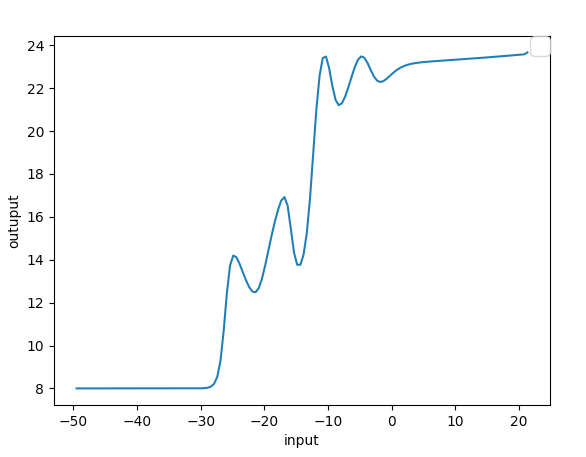
\includegraphics[width=10cm]{asset/boston_0000001_SGDkaiming_normal__non_200_function_2.png}
            \caption{活性化関数の形}
            \label{boston}
    \end{center}
\end{figure}


\section{実験3の結果 K-AFの性能が上がる条件探査}
\label{evo3}
\ref{exp3}で示した比較実験の結果を記述する。
wine及びbostonのデータセットで最も性能が良かったニューラルネットワークの設定のトップ5を記述する。

\subsubsection{wineの場合}

\begin{table}[htbp]
    \begin{center}
        \caption{wineを推論するときの最もいい設定}
        \label{winebest}
        \vspace{2mm} 
        \begin{tabular}{ |c|c|c| }
        組み合わせ & Acc & エラーの回数 \\
        \hline
        iris           & $ 10^{-3} $    & 3 \\
        digits         & $ 10^{-3} $    & 3 \\
        wine           & $ 10^{-3} $    & 3 \\
        boston         & $ 10^{-3} $    & 13  \\
        breast\_cancer & $ 10^{-3} $    & 30 \\
        \end{tabular}
    \end{center}
\end{table}

表\ref{winebest}を参考にすると

\subsubsection{bostonの場合}

\begin{table}[htbp]
    \begin{center}
        \caption{bostonを推論するときの最もいい設定}
        \label{bostonbest}
        \vspace{2mm} 
        \begin{tabular}{ |c|c|c| }
        組み合わせ & Acc & エラーの回数 \\
        \hline
        iris           & $ 10^{-3} $    & 3 \\
        digits         & $ 10^{-3} $    & 3 \\
        wine           & $ 10^{-3} $    & 3 \\
        boston         & $ 10^{-3} $    & 13  \\
        breast\_cancer & $ 10^{-3} $    & 30 \\
        \end{tabular}
    \end{center}
\end{table}




\subsection{性能評価まとめ}
wineとbostonの結果をまとめるとと言うことがわかった。


\section{まとめ}

K-AFの精度、勾配消失の有無、実用性の観点から先行研究との比較を行った。
実験結果を踏まえ, 第 6 章で解決した課題をまとめ、将来への展望を述べる。


%%% Local Variables:
%%% mode: japanese-latex
%%% TeX-master: "./thesis"
%%% End:
